\documentclass[12pt]{article}
\usepackage{stmaryrd}
\usepackage{graphicx}
\usepackage[utf8]{inputenc}

\usepackage[french]{babel}
\usepackage[T1]{fontenc}
\usepackage{hyperref}
\usepackage{verbatim}

\usepackage{color, soul}

\usepackage{pgfplots}
\pgfplotsset{compat=1.15}
\usepackage{mathrsfs}

\usepackage{amsmath}
\usepackage{amsfonts}
\usepackage{amssymb}
\usepackage{tkz-tab}
\author{Destiné aux élèves de Terminale S\\Lycée de Dindéfelo\\Présenté par M. BA}
\title{\textbf{Calcul Intégral Ts2}}
\date{\today}
\usepackage{tikz}
\usetikzlibrary{arrows, shapes.geometric, fit}

% Commande pour la couleur d'accentuation
\newcommand{\myul}[2][black]{\setulcolor{#1}\ul{#2}\setulcolor{black}}
\newcommand\tab[1][1cm]{\hspace*{#1}}

\begin{document}
\maketitle
\newpage
\section*{\underline{\textbf{\textcolor{red}{I. Primitive }}}}
\subsection*{\underline{\textbf{\textcolor{red}{1. Définition}}}}
Soit $I$ un intervalle de $\mathbb{R}$  et  f une fonction continue sur I. On dit que F est une primitive de f sur $I$ notée $\int f $ si,\\ $F$ est dérivable sur $I$ et $\forall x \in I$, F'(x)=f(x)
\subsection*{\underline{\textbf{\textcolor{red}{Exemple}}}}
Soit $f$  et  $F$ deux fonctions définies par : 
\subsection*{\underline{\textbf{\textcolor{red}{Théorème 1}}}}
Toute fonction continue sur $I$ y admet une primitive.
\subsection*{\underline{\textbf{\textcolor{red}{Théorème 2}}}}
Si $F$ est une primitive de $f$ sur $I$, alors toute fonction $G$ définie par
$G(x)=F(x)+c$;c une constante est aussi une primitive de $f$ sur $I$.
 
Donc deux primitives quelconques d'une fonction diffèrent d'une constante et il existe une unique primitive qui prend une valeur $y$ en $x_{0}$.
\subsection*{\underline{\textbf{\textcolor{red}{Théorème 3}}}}

Soit $f$ une fonction dérivable sur $I$ de dérivée $f'$ continue sur $I$ et $g$ une fonction continue sur $I$ de primitive $G$ définie sur un intervalle $J$ contenant $f(I)$, alors $(g\circ f)f'$ a pour primitive sur $I$, $G\circ f$.
\subsection*{\underline{\textbf{\textcolor{red}{2. Opération sur les primitives}}}}
Si F est une primitive de f et G une primitive de g, alors 

$\alpha F+\beta G$ est une primitive de $\alpha f+\beta g$;$\alpha $, $\beta \in \mathbb{R}$
\subsection*{\underline{\textbf{\textcolor{red}{Tableau de quelques primitives}}}}
u et v sont deux fonctions continues et c une constante.

\begin{minipage}[t]{0.5\textwidth}
\centering
\begin{tabular}{|c|c|}
\hline
$f$ & $F$\\
\hline
$\alpha \in \mathbb{R}$ & $ax+c$\\
\hline
$\frac{1}{x};x>0$ & $\ln(x)+c$\\
\hline
$e^{x}$ & $e^{x}$\\
\hline
$\sin x$ & $-\cos x +c$\\
\hline
$\cos x$ & $-\sin x +c$\\
\hline
$\frac{1}{\sqrt{x}}; x>0$ & $2\sqrt{x}$\\
\hline
$\frac{1}{x^{2}}; x>0$ & $-\frac{1}{x}$\\
\hline
\end{tabular}
\end{minipage}%
\begin{minipage}[t]{0.5\textwidth}
\centering
\begin{tabular}{|c|c|}
\hline
$f$ & $F$\\
\hline
$\alpha \in \mathbb{R}$ & $ax+c$\\
\hline
$x^{n}$ & $\frac{x^{n+1}}{n+1}+c$\\
\hline
$\frac{1}{\cos^{2} x}=1+\tan^{2} x$ & $\tan x$\\
\hline
$u'u^{n}$ & $\frac{u^{n+1}}{n+1}$\\
\hline
$\frac{u'}{u}$ & $\ln(|u|)$\\
\hline
$u'e^{u}$ & $e^{u}$\\
\hline
$\frac{u'}{u^{2}}$ & $-\frac{1}{u}$\\
\hline
\end{tabular}
\end{minipage}

\begin{tabular}{|c|c|}
\hline
$f$ & $F$\\
\hline
$u'\cos u$ & $\sin u$\\
\hline
$u'\sin u$ & $-\cos u$\\
\hline
$\frac{u'}{\cos^{2} u}=1+\tan^{2} u$ & $\tan u$\\
\hline
$\frac{u'}{\sqrt{u}}$ & $2\sqrt{u}$\\
\hline
$u'v+v'u$ & $uv$\\
\hline
$\lambda f; \lambda \in \mathbb{R}$ & $\lambda F$\\
\hline
$\frac{u'v+v'u}{v^{2}}$ & $\frac{u}{v}$\\
\hline
\end{tabular}
\subsection*{\underline{\textbf{\textcolor{red}{Théorème }}}}
Si $u$ et $v$ sont dérivables sur $I$ de dérivées $u'$ et $v'$ continues sur $I$, alors
$\int u'v=uv-\int uv'$ En effet, $(uv)'=u'v+v'u \Longrightarrow u'v=(uv)'-uv'$

$\Longrightarrow \int u'v=\int (uv)'-\int uv'$ 

$\Longrightarrow \int u'v=uv-\int uv'$ 
\subsection*{\underline{\textbf{\textcolor{red}{Exemple}}}}
Déterminer les primitives de :

$f(x)=x\cos x$ ; $g(x)=xe^{x}$ ; $h(x)=\ln x$
\subsection*{\underline{\textbf{\textcolor{red}{Résolution }}}}
\subsection*{\underline{\textbf{\textcolor{red}{II. Définition et propriétés}}}}
\subsection*{\underline{\textbf{\textcolor{red}{1. Définition }}}}
Soit $I$ un intervalle de $\mathbb{R}$, $a$, $b$ $\in I$ et $f$ une fonction continue sur $I$. On appelle intégrale de $a$ à $b$ de $f$ le réel noté

$\int_{a}^{b}f(x)dx=[F(x)]_{a}^{b}=F(b)-F(a)$ où $F$ est une primitive quelconque de $f$ sur 
$[a,b]$ ou $[b,a]$
\subsection*{\underline{\textbf{\textcolor{red}{Remarques }}}}
\begin{itemize}
\item[•] Le choix de la primitive $F$ n'influe pas le résultat de l'intégrale. En effet, si $F$ et $G$ sont deux primitives d'une même fonction $f$ sur $I$, alors elles différent d'une constante. Les quantités $F(b)-F(a)$ et $G(b)-G(a)$ sont donc égales.

Soit $G(x)=F(x)+c$, alors \[\int_{a}^{b}f(x)dx=[G(x)]_{a}^{b}
=G(b)-G(a)=F(b)+c-(F(a)+c)=F(b)-F(a)\]
\item[•] Soit $I$ un intervalle et $x_{0}\in I$ pour tout réel $x$ de $I$, nous avons:
		\[\int_{x_{0}}^{x}f(t)dt=[F(t)]_{x_{0}}^{x}=F(x)-F(x_{0})\]
La fonction \texttt{F} définie sur $I$ par \[\texttt{F}=\int_{x_{0}}^{x}f(t)dt\]
est donc la primitive de f sur $I$ qui s'annule en $x_{0}$.
\item[•] La lettre t (ou x) choisie pour la variable est une variable "muette" ; elle peut être notée par toute autre lettre. Ce qui signifie que :
\[\int_{a}^{b}f(x)dx=\int_{a}^{b}f(t)dt=\int_{a}^{b}f(u)du=F(b)-F(a) \]
\end{itemize}
\subsection*{\underline{\textbf{\textcolor{red}{Exemple  }}}}
Calculer
\[I=\int_{4}^{5}\frac{1}{x^{2}-9}dx , J=\int_{0}^{1}\frac{x}{x+1}dx, K=\int_{1}^{e}\frac{\ln x}{x}dx\]
\subsection*{\underline{\textbf{\textcolor{red}{Résolution }}}}
\subsection*{\underline{\textbf{\textcolor{red}{2. Propriétés }}}}
Soit $I$ un intervalle de $\mathbb{R}, a, b, c, \in I, f$ et $g$ deux fonctions continues sur $I, \alpha, \beta \in \mathbb{R},$ alors
\begin{itemize}
\item[•] \[\int_{a}^{a}f(x)dx=0\]
\item[•] \[\int_{a}^{b}f(x)dx=-\int_{b}^{a}f(x)dx\]
\item[•] Relation de Chasles \[\int_{a}^{b}f(x)dx=\int_{a}^{c}f(x)dx+\int_{c}^{b}f(x)dx\]
\item[•] Linéarité de l'intégration \[\int_{a}^{b}(\alpha f+\beta g)(x)dx=
\alpha \int_{a}^{b}f(x)dx+\beta\int_{a}^{b}g(x)dx \]
\item[•] Si $f$ est paire, alors \[\int_{-a}^{a}f(x)dx=2\int_{0}^{a}f(x)dx \]
\item[•] Si $f$ est impaire, alors \[\int_{-a}^{a}f(x)dx=0\]
\item[•] Si $f$ est périodique de période $T$, alors
\[\int_{a}^{a+T}f(x)dx=\int_{0}^{T}f(x)dx\]
\item[•] Positivité de l'intégration : si $a\leq b$ et $f\geq 0$ sur $[a, b]$, alors
\[\int_{a}^{b}f(x)dx\geq 0\]
\item[•] Conservation de l'ordre de l'intégration : $a\leq b$ et $f\geq g$ sur $[a, b]$, alors \[\int_{a}^{b}f(x)dx\geq \int_{a}^{b}g(x)dx \]
\item[•] \[\mid\int_{a}^{b}f(x)dx\mid\leq \int_{a}^{b}g(x)dx \]
\item[•]  Inégalité de la moyenne : La fonction $f$ étant continue sur $[a, b]$, alors il existe deux réels $m$ et $M$ tels que, pour tout réel $x\in [a, b]$ on ait $m\leq f(x)\leq M$ et donc : \[m(b-a)\leq \int_{a}^{b}f(x)dx \leq M(b-a)\] 
En effet
\[m\leq f(x)\leq M \Longrightarrow \int_{a}^{b}mdx \leq \int_{a}^{b}f(x)dx \leq \int_{a}^{b}Mdx \Longrightarrow m(b-a)\leq \int_{a}^{b}f(x)dx \leq M(b-a)\]
\end{itemize}
\subsection*{\underline{\textbf{\textcolor{red}{Théorème de la moyenne }}}}
Pour toute fonction $f$ définie et continue sur l'intervalle $[a, b]$, d'après le théorème des valeurs intermédiaires, il existe au moins un réel $c\in [a, b]$ tel que
\[f(c) =\frac{1}{b-a}\int_{a}^{b}f(x)dx \]
Le réel $f(c)$ est appelé valeur moyenne de $f$ sur $[a, b]$.
\subsection*{\underline{\textbf{\textcolor{red}{Interprétations géométriques }}}}
Le plan est muni d'un repère orthogonal  $O,\vec{i},\vec{j}.$ Soit f une fonction continue et positive de courbe représentative $C_{f}$, alors
\begin{itemize}
\item[•] L'encadrement \[m(b-a)\leq \int_{a}^{b}f(x)dx \leq M(b-a)\] signifie que l'aire du domaine coloré est minorée par l'aire du rectangle $ABCD$, et majorée par celle du rectangle $ABEF$
\item[•]  L'égalité \[f(c) =\frac{1}{b-a}\int_{a}^{b}f(x)dx \] signifie que l'aire du domaine coloré est égale à celle du rectangle $ABGH$

\begin{center}
   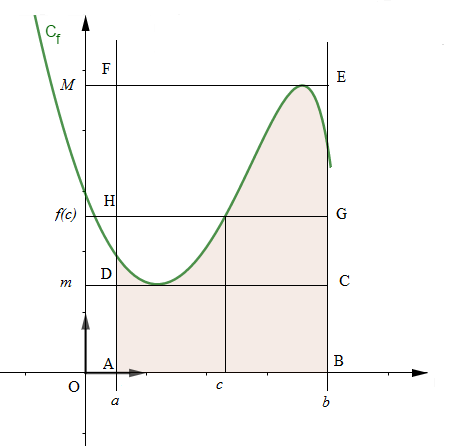
\includegraphics[scale=0.5]{surface1.png}
\end{center}

\end{itemize}
\subsection*{\underline{\textbf{\textcolor{red}{Exercice d'application }}}}
Soit la suite $(u_{n})$ définie par $u_{n}=\int_{1}^{e}x(\ln x)^{n}dx$

Montrer que $u_{n}$ est décroissante
\subsection*{\underline{\textbf{\textcolor{red}{Résolution  }}}}
\subsection*{\underline{\textbf{\textcolor{red}{III. Méthodes d'intégration }}}}
\subsection*{\underline{\textbf{\textcolor{red}{1. A l'aide du tableau de primitives }}}}
\subsection*{\underline{\textbf{\textcolor{red}{Exemple  }}}}
Calculer \[I=\int_{0}^{1}x\sqrt{1-x^{2}}dx, J=\int_{0}^{\frac{\pi}{6}}\sin 2x \cos 3x dx\]
\subsection*{\underline{\textbf{\textcolor{red}{2. A l'aide de la linéarisation }}}}
\subsection*{\underline{\textbf{\textcolor{red}{Exemple}}}}
Calculer \[I=\int_{0}^{\pi}\sin^{5} x dx \]
\subsection*{\underline{\textbf{\textcolor{red}{3. Par changement de variables}}}}
\subsection*{\underline{\textbf{\textcolor{red}{Théorème}}}}
Si $g$ est continue sur $[a,b]$ et de dérivée $g'$ continue sur $[a,b]$.

Si $f$ est continue sur $[\alpha,\beta]$ avec $\alpha = g(a)$ et $\beta=g(b)$, alors
\[ \int_{a}^{b}f\circ g(x)g'(x)dx=\int_{\alpha}^{\beta}f(u)du \]
\subsection*{\underline{\textbf{\textcolor{red}{Exemple}}}}
Calculer \[A=\int_{0}^{\frac{\pi}{4}}\tan x dx, B=\int_{0}^{\pi}\sin x \cos^{4} x dx\]
\subsection*{\underline{\textbf{\textcolor{red}{Résolution}}}}
\subsection*{\underline{\textbf{\textcolor{red}{Remarque}}}}
\[\int_{a}^{b}\alpha f(\alpha t+\beta)dt=\int_{\alpha a+\beta}^{\alpha b+\beta}f(u)du\]
$u=\alpha t +\beta \Rightarrow du=\alpha dt$
\subsection*{\underline{\textbf{\textcolor{red}{4. Intégration par parties}}}}
Si $u$ et $v$ sont dérivables sur $I$ de dérivées u' et v' continues sur $I$ et $a$, $b \in I$ alors
\[\int_{a}^{b}u'(x)v(x)dx=[u(x)v(x)]_{a}^{b}-\int_{a}^{b}u(x)v'(x)dx\]
\subsection*{\underline{\textbf{\textcolor{red}{Exemple}}}}
Calculer les intégrales suivantes 
\[A=\int_{0}^{\pi}x\cos xdx, B=\int_{1}^{e}x\ln x dx\]
\subsection*{\underline{\textbf{\textcolor{red}{Résolution}}}}

\subsection*{\underline{\textbf{\textcolor{red}{IV. Calcul d'aire et de volume }}}}
\subsection*{\underline{\textbf{\textcolor{red}{1. Calcul d'aires}}}}

Soit $(O ; \vec{i} ; \vec{j})$ un repère orthogonale, $||\vec{i}||=m$ cm, $||\vec{j}||=n$ cm.

L'unité d'aire est l'aire du quadrilatère construit sur les vecteurs de bases du repères.

1 unité d'aire $(u.a)=m\times n$ $cm^{2}$

\begin{center}
   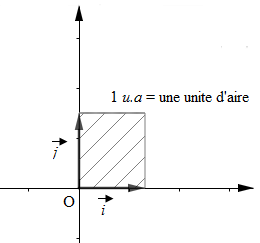
\includegraphics[scale=0.5]{surface2.png}
\end{center}
\begin{itemize}
\item[•] Soit $f\geq 0$ sur [a, b].

L'aire $\mathcal{A}$  de la partie du plan comprise entre $C_{f}$,l'axe des abscisses et les droites d'équation $x=a$ et $x=b$est égale à:
\[\mathcal{A}=\int_{a}^{b}f(x)dx\quad u.a\]
\end{itemize}
\subsection*{\underline{\textbf{\textcolor{red}{Exemple }}}}
Soit $(O ; \vec{i} ; \vec{j})$ un repère orthogonale, $||\vec{i}||=||\vec{j}||=1$ cm. On Considère la parabole $C_{f}$ représentant la fonction $f$ définie sur $\mathbb{R}$ par $f(x)=x^{2}$.

Calculer l'aire $\mathcal{A}$ en $cm^{2}$ du domaine délimité par $C_{f}$, l'axe des abscisses et les droites d'équation $x=-1$ et $x=2$
\subsection*{\underline{\textbf{\textcolor{red}{Résolution}}}}
\begin{eqnarray}
\mathcal{A} &=& \int_{-1}^{1}|f(x)-g(x)|\mathrm{d}x \nonumber \\
            &=& \int_{-1}^{1}|\mathrm{e}^{x}-1|\mathrm{d}x \nonumber \\
            &=& \int_{-1}^{0}-(\mathrm{e}^{x}-1)\mathrm{d}x+\int_{0}^{1}\mathrm{e}^{x}-1\mathrm{d}x \nonumber \\
            &=& -[\mathrm{e}^{x}-x]_{-1}^{0}+[\mathrm{e}^{x}-x]_{0}^{1} \nonumber \\
            &=& -\left[1-\dfrac{1}{\mathrm{e}}-1\right]+[\mathrm{e}-1-1] \nonumber \\
            &=& \dfrac{1}{\mathrm{e}}+\mathrm{e}-2 \nonumber
\end{eqnarray}

\begin{center}
    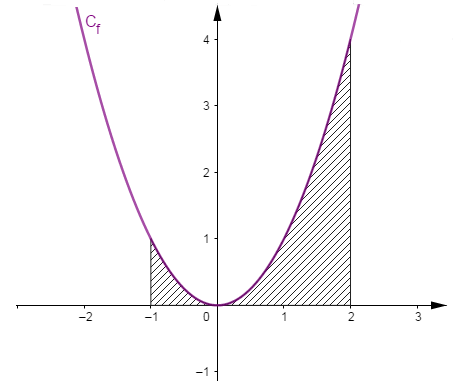
\includegraphics[width=200pt]{surface3.png}
\end{center}

Soit $f$ une fonction continue sur $[a, b]$ et $D$ une droite d'équation $\alpha x + \beta.$

L'aire de la partie du plan comprise entre $C_{f}$, $D$ et les droites d'équation $x=a$ et $x=b$ est égale à :
$$\int_{a}^{b}|f(x)-(\alpha x+\beta)|\mathrm{d}x\;u.a$$

\begin{center}
   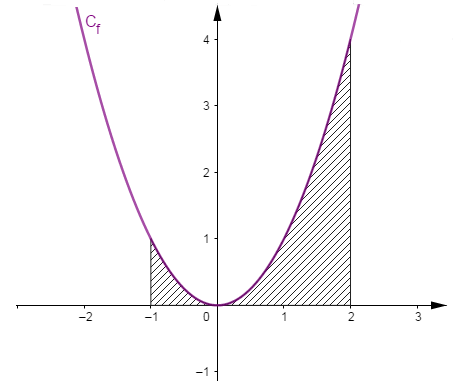
\includegraphics[scale=0.5]{surface3.png}
\end{center}
\begin{itemize}
\item[•] Soit $f\geq 0$ sur [a, b].

L'aire $\mathcal{A}$  de la partie du plan comprise entre $C_{f}$,l'axe des abscisses et les droites d'équation $x=a$ et $x=b$est égale à:
\[\mathcal{A}=\int_{a}^{b}-f(x)dx\quad u.a\]
\end{itemize}
\subsection*{\underline{\textbf{\textcolor{red}{Exemple}}}}
Soit $f$ la fonction définie sur $\mathbb{R}$ par $f(x)=-x^{2}$.

Calculer l'aire $\mathcal{A}$ du domaine délimité par $C_{f}$,l'axe des abscisses et les droites d'équation $x=-1$ et $x=2$
\subsection*{\underline{\textbf{\textcolor{red}{Résolution}}}}
\begin{eqnarray}
\mathcal{A} &=& \int_{-1}^{2}-f(x)\mathrm{d}x \nonumber \\
            &=& \int_{-1}^{2}x^{2}\mathrm{d}x \nonumber \\
            &=& \left[\dfrac{x^{3}}{3}\right]_{-1}^{2} \nonumber \\
            &=& \dfrac{8}{3} - \dfrac{(-1)^{3}}{3} \nonumber \\
            &=& \dfrac{8}{3} + \dfrac{1}{3} \nonumber \\
            &=& 3\; \text{cm}^{2} \nonumber
\end{eqnarray}
\begin{center}
    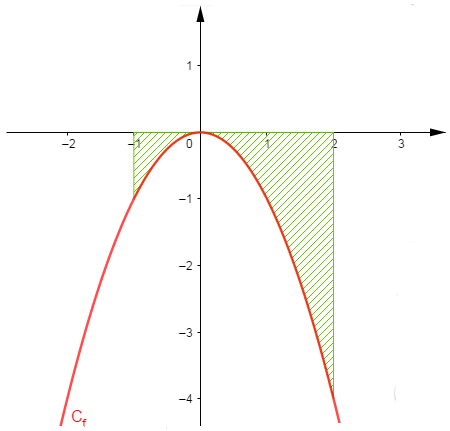
\includegraphics[scale=0.5]{surface4.png}
\end{center}
\begin{itemize}
\item[•] Soit $f$ et $g$ deux fonctions continues sur [a, b]

L'aire de la partie du plan comprise entre $C_{f}$, $C_{g}$ et les droites d'équation $x=a$ et $x=b$ est égale à :
\[\int_{a}^{b}|f(x)-g(x)|dx\quad u.a\]
\end{itemize}
\subsection*{\underline{\textbf{\textcolor{red}{Exemple : cas particulier d'une fonction changeant de signe}}}}
Soit $f$ et $g$ les fonctions définies sur $\mathbb{R}$ par $f(x)=e^{x}-1$ et $g(x)=0$

Calculer l'aire $\mathcal{A}$ du domaine délimité par $C_{f}$, $C_{g}$ et les droites d'équation $x=-1$ et $x=1$
\subsection*{\underline{\textbf{\textcolor{red}{Résolution}}}}
\begin{eqnarray}
\mathcal{A} &=& \int_{-1}^{1}|f(x)-g(x)|\mathrm{d}x \nonumber \\
            &=& \int_{-1}^{1}|\mathrm{e}^{x}-1|\mathrm{d}x \nonumber \\
            &=& \int_{-1}^{0}-(\mathrm{e}^{x}-1)\mathrm{d}x+\int_{0}^{1}\mathrm{e}^{x}-1\mathrm{d}x \nonumber \\
            &=& -[\mathrm{e}^{x}-x]_{-1}^{0}+[\mathrm{e}^{x}-x]_{0}^{1} \nonumber \\
            &=& -\left[1-\dfrac{1}{\mathrm{e}}-1\right]+[\mathrm{e}-1-1] \nonumber \\
            &=& \dfrac{1}{\mathrm{e}}+\mathrm{e}-2 \nonumber
\end{eqnarray}


    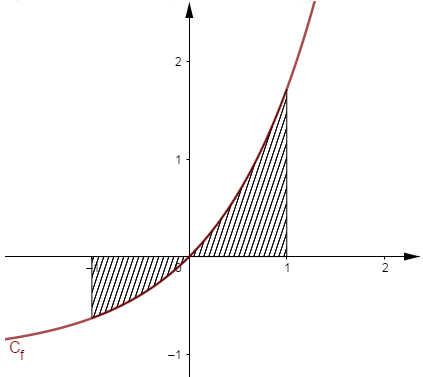
\includegraphics[width=200pt, height=200pt]{aire2.png}


$\centerdot$ Soit $f$ une fonction continue sur $[a, b]$ et $D$ une droite d'équation $\alpha x + \beta.$

L'aire de la partie du plan comprise entre $C_{f}$, $D$ et les droites d'équation $x=a$ et $x=b$ est égale à :
$$\int_{a}^{b}|f(x)-(\alpha x+\beta)|\mathrm{d}x\;u.a$$

\subsection*{\underline{\textbf{\textcolor{red}{Exemple }}}}
Soit $f$ la fonction définie sur $\mathbb{R}_{+}$ par $f(x)=\sqrt{x}$ et $D$ et les droites d'équation $x=\frac{1}{2}$ et $x=2$ 
\[\mathcal{A}=\int_{\frac{1}{2}}^{2}|f(x)-(\alpha x+\beta)|dx\]
\[=\int_{\frac{1}{2}}^{2}(x+\frac{1}{2}-\sqrt{x})dx\]
\[= \left[ \frac{x^{2}}{2}+\frac{1}{2}x-\frac{x^{\frac{3}{2}}}{\frac{3}{2}} \right]_{\frac{1}{2}}^{2}  \]
\[=3-\frac{3}{8}-\frac{7\sqrt{2}}{6}\]
\begin{center}
    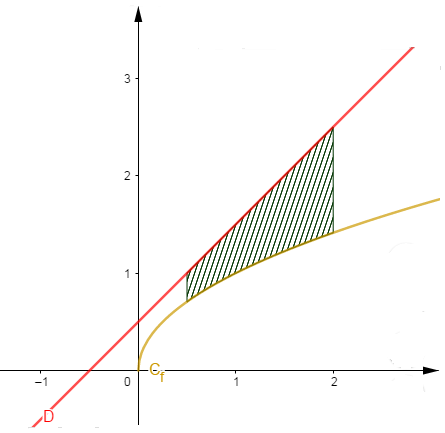
\includegraphics[scale=0.5]{surface5.png}
\end{center}
\subsection*{\underline{\textbf{\textcolor{red}{IV.2 Calcul de volume}}}}
Soit $(O\;;\ \vec{i}\;,\ \vec{j}\;,\ \vec{k})$ un repère orthogonal.

L'unité de volume est le volume du parallélépipède construit sur les vecteurs de bases du repères.
\begin{center}
    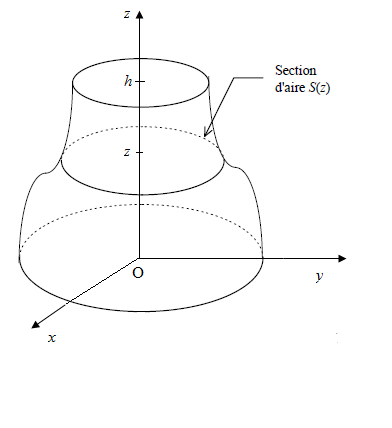
\includegraphics[scale=0.5]{tronc.png}
\end{center}
Soit $S$ un solide de hauteur $h$. Un plan $\mathcal{P}$ parallèle au plan $(x'Ox)$ coupe $S$ suivant une figure plane de surface $S(z)$. Le volume $\mathcal{V}$ de $S$ est égal à 
$$\mathcal{V}=\int_{0}^{h} S(z) \, \mathrm{d}z \; u.v.$$

$1\;u.v = \text{une unité de volume}$

\begin{center}
    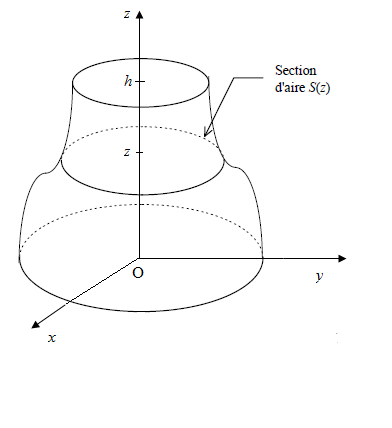
\includegraphics[scale=0.5]{tronc.png}
\end{center}

\section*{Exemples}

\subsection*{a) Cylindre $(R, h)$}

$S(z)=\pi R^{2}$
\begin{eqnarray*}
\mathcal{V} &=& \int_{0}^{h} S(z) \, \mathrm{d}z \\
            &=& \int_{0}^{h} \pi R^{2} \, \mathrm{d}z \\
            &=& \left[\pi R^{2}z \right]_{0}^{h} \\
            &=& \pi R^{2}h
\end{eqnarray*}

\begin{center}
   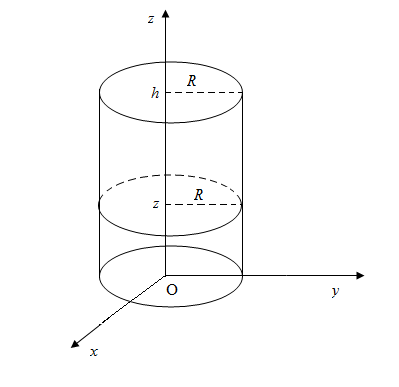
\includegraphics[scale=0.5]{cylindre.png}
\end{center}

\subsection*{b) Cône $(R, h)$}

$S(z)=\pi r^{2}$, d'après Thalès $\dfrac{r}{R}=\dfrac{z}{h}$, donc $S(z)=\pi\dfrac{R^{2}}{h^{2}}z^{2}.$

Donc 

\begin{eqnarray*}
\mathcal{V} &=& \int_{0}^{h} S(z) \, \mathrm{d}z \\
            &=& \int_{0}^{h} \pi \dfrac{R^{2}}{h^{2}} z^{2} \, \mathrm{d}z \\
            &=& \pi \dfrac{R^{2}}{h^{2}} \int_{0}^{h} z^{2} \, \mathrm{d}z \\
            &=& \pi \dfrac{R^{2}}{h^{2}} \left[\dfrac{z^{3}}{3}\right]_{0}^{h} \\
            &=& \pi \dfrac{R^{2} h}{3}
\end{eqnarray*}

\begin{center}
    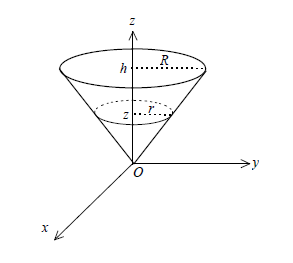
\includegraphics[scale=0.5]{cone.png}
\end{center}

\subsection*{c) Sphère de rayon $R$}

$S(z)=\pi r^{2}$ or $r^{2}+z^{2}=R^{2}\ \Rightarrow\ r^{2}=R^{2}-z^{2}$, donc $S(z)=\pi(R^{2}-z^{2}).$

Alors

\begin{eqnarray*}
\mathcal{V} &=& \int_{-R}^{R} S(z) \, \mathrm{d}z \\
            &=& \int_{-R}^{R} \pi (R^{2}-z^{2}) \, \mathrm{d}z \\
            &=& 2\pi \int_{0}^{R} (R^{2}-z^{2}) \, \mathrm{d}z \\
            &=& 2\pi \left[R^{2}z - \dfrac{z^{3}}{3}\right]_{0}^{R} \\
            &=& 2\pi \left(R^{3} - \dfrac{R^{3}}{3}\right) \\
            &=& \dfrac{4}{3}\pi R^{3}
\end{eqnarray*}

\begin{center}
    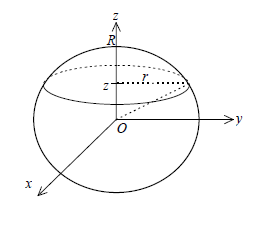
\includegraphics[scale=0.5]{spher.png}
\end{center}

\subsection*{Remarque}

Soit $f$ une fonction continue sur $[a, b]$, alors le volume engendré par la rotation de $C_{f}$, $x=a$ et $x=b$ autour de l'axe des abscisses est égal à 
$$\mathcal{V}=\int_{a}^{b} \pi (f(x))^{2} \, \mathrm{d}x$$ 
\end{document}